\usepackage{enumitem}
% SELBST: tikz for drawing
\usepackage{tikz}
\usepackage{tabularx}
\usepackage{multirow}
\usepackage{pgfplots}
\pgfplotsset{compat=1.17}
\usepackage{pgf-pie}
\usepackage{subfigure}
\usepackage{subcaption}


%% The first command in your LaTeX source must be the \documentclass command.
\documentclass[sigconf]{acmart}
\settopmatter{printacmref=false}
%%
%% \BibTeX command to typeset BibTeX logo in the docs
\AtBeginDocument{%
  \providecommand\BibTeX{{%
    \normalfont B\kern-0.5em{\scshape i\kern-0.25em b}\kern-0.8em\TeX}}}

% TODO
%% Rights management information.  This information is sent to you
%% when you complete the rights form.  These commands have SAMPLE
%% values in them; it is your responsibility as an author to replace
%% the commands and values with those provided to you when you
%% complete the rights form.
\setcopyright{iw3c2w3}
\copyrightyear{\the\year{}}
\acmYear{\the\year{}}

\begin{document}

\title[Prompting Behavior in Text-prompt-based Generative Model Interactions]{Exploring User
Prompting Behavior in Text-prompt-based Generative Model Interactions}

\author{Maximilian Slapnik}
%\orcid{1234-5678-9012}
\email{Maximilian.Slapnik@campus.lmu.de}
\affiliation{%
  \institution{LMU Munich}
  \city{Munich}
  \country{Germany}
}

%%%%%%%%%%%%%%%%%%%%%%%%%%%%%%%%%%%%%%% ABSTRACT

\begin{abstract}
  \sloppy
  Artificial Intelligence (AI) plays an increasingly important role in the daily lives of
  millions of people.
  Large Language Models (LLMs) and text-to-image generation tools are one of the most prominent
  implementations of AI that are used
  not only by experts, but equally by ordinary users as well.
  LLMs can respond to any textual input (prompts) with human-like answers, leveraging the
  training data that was used to implement the model.
  Even though prompting LLMs may seem very straightforward, the question arises if it is possible
  to streamline the interactions with said models in order to optimize outputs.
  We investigate user behavior in interactions with LLMs based on a randomized trial of 100
  samples that are publicly available on the platforms ShareGPT and Midjourney.
  The goal of this analysis is the discovery of recurring patterns as well as the
  evaluation of human tendencies and biases when interacting with AI models in
  order to understand prevalent behaviors and explore optimization opportunities.
\end{abstract}

%%%%%%%%%%%%%%%%%%%%%%%%%%%%%%%%%%%%%%% CCS CONCEPTS

%% code below is generated by the tool at http://dl.acm.org/ccs.cfm.

\begin{CCSXML}
  <ccs2012>
  <concept>
  <concept_id>10003120.10003123</concept_id>
  <concept_desc>Human-centered computing~Interaction design</concept_desc>
  <concept_significance>500</concept_significance>
  </concept>
  <concept>
  <concept_id>10002951.10003317</concept_id>
  <concept_desc>Information systems~Information retrieval</concept_desc>
  <concept_significance>300</concept_significance>
  </concept>
  <concept>
  <concept_id>10010147.10010178.10010179</concept_id>
  <concept_desc>Computing methodologies~Natural language processing</concept_desc>
  <concept_significance>300</concept_significance>
  </concept>
  </ccs2012>
\end{CCSXML}

\ccsdesc[500]{Human-centered computing~Interaction design}
\ccsdesc[300]{Infor-mation systems~Information retrieval}
\ccsdesc[300]{Computing methodo-logies~Natural language processing}

%%%%%%%%%%%%%%%%%%%%%%%%%%%%%%%%%%%%%%% KEYWORDS

\keywords{Large Language Models, user behavior, prompting, interaction patterns}

%%%%%%%%%%%%%%%%%%%%%%%%%%%%%%%%%%%%%%% TITLE

\maketitle


%%%%%%%%%%%%%%%%%%%%%%%%%%%%%%%%%%%%%%% CHAPTERS

%%%%%%%%%%%%%%%%%%%%%%%%%%%%%%% INTRODUCTION %%%%%%%%%%%%%%%%%%%%%%%%%%%%%%%

%%%%%%%%%%%%%%%%%%%%%%%%%%%%%%%%% Introduction %%%%%%%%%%%%%%%%%%%%%%%%%%%%%%%%%
\section{Introduction}
\label{sec:introduction}
%% refer to https://intra.ece.ucr.edu/~rlake/Whitesides_writing_res_paper.pdf for tips on introduction?
%% INTRO - TOPIC

%Why is the work important?
\sloppy % use sloppy to improve linebreaks - longer words do not overflow
Artificial Intelligence (AI) -based tools continually gain prominence as regularly leveraged tools in the
daily lives of millions of people.
Today, the significance of this technology is reflected in the current AI market size that is
estimated to be \$142 billion USD, and forecasted to increase more than tenfold by 2030~\cite{statista_artificial_2023}.
% TODO include some stats, such as daily ChatGPT users?
In addition to typical AI applications such as recommendation systems or autonomous agents, generative
models are notably increasing in popularity as well, making it one of the central research topics
in the field.
One of the most widely used implementations of generative models are Large Language Models (LLMs),
the most popular example at the moment being OpenAI's ChatGPT~\cite{openai_chatgpt_2023}.
Adoption rates of generative AI applications among professionals are increasing rapidly, and are
already at
around 30\%~\cite{statista_us_2022}.

Large Language Models are mainly implemented in the form of text generating chatbots that can
answer seemingly any question a user might pose.
Although no expert knowledge is required to formulate a prompt and interact with an LLM-based bot, it is challenging to optimize the output, since it varies depending on the structure, wording,
and composition of the input. %TODO cite?
Any form of model input, whether it is in the form of a task or a question, is commonly
referred to as \("\)prompting\("\) the model.
Due to the vast application possibilities and promising future developments of LLMs, exploration of
user prompting behavior in interactions with such models is of particular interest.
Plenty of research has been conducted in the field of user interactions with LLMs already,
mainly in regard to query reformulation strategies, studies of common user errors when prompting,
different prompt composition strategies, and general LLM limitations.

%- The objectives of the work.
In this paper, we are going to explain the fundamentals and workings of LLMs and prompting,
describe related research in the realm of user - LLM exchange, and perform our own investigation of
user behavior in such interactions.
This investigation has the objective of facilitating comprehension of existing challenges users
face when dealing with Large Language Models.
Furthermore, readers will gain a better understanding of the design of effective prompts that
enhance model output.

%- Guidance to the reader:
% What should the reader watch for in the paper?
% What are the interesting high points? What strategy did we use?
Since the main part of this paper will be complemented by an analysis of real-world examples, the
reader can expect to develop an enhanced comprehension of actual user prompting behavior.
To obtain these insights, we will leverage input data mainly gathered from the website
ShareGPT~\cite{sharegpt_sharegpt_2023},
which enables users to store conversations they have had with the ChatGPT model for later retrieval
or sharing them publicly.

% TODO add links (\ref) to sections
The paper is organized as follows.
This introduction is succeeded by a related work section that sets the context for all subsequent
parts by first focusing on Large Language Models (LLMs) and covering general information about
their workings, training data, text generation capabilities, real-world usage, and current limitations.
We then explore user interactions with LLMs, explain the concept of prompting, and highlight
various use cases as well as related research.

The next section introduces the study by outlining the research objective and
describing the methodology and individual steps that will be taken.
It then focuses on the research method we use, as well as the ShareGPT and Midjourney platforms,
which provide the input data for the study.

Subsequently, we present our findings.
To do so, we first list the study results, organized into predefined categories.
% TODO check if true
We then analyze observable trends in user behavior and data patterns.

The following discussion section starts with a synthesis of our observations.
We then go into more detail about the reasons why users interact with LLMs the way they do,
offering reasoning and informed assumptions.
Additionally, we explore possibilities for prompt improvements based on findings from related
research.

In the outlook section, we provide a perspective on future developments, divided into an
introduction of the concept of Auto-GPT as a possible future iteration of prompting, as well as an
overview of prompt engineering as a newly emerging discipline in the technology sector.

The final section of this paper offers a consolidation of the findings and associated discussions,
as well as a summary of how we could recognize findings from related research in our own input
samples.

%%%%%%%%%%%%%%%%%%%%%%%%%%%%%%% BACKGROUND %%%%%%%%%%%%%%%%%%%%%%%%%%%%%%%

%%%%%%%%%%%%%%%%%%%%%%%%%%%%%%%%% Background %%%%%%%%%%%%%%%%%%%%%%%%%%%%%%%%%
\section{Background}
\label{sec:background}

%%%%%%%%%%%%%%%%%%%%%%%%%%%%%%%%% LLMs %%%%%%%%%%%%%%%%%%%%%%%%%%%%%%%%%%%%

\subsection{Large Language Models (LLMs)}
\label{subsec:large-language-models-(llms)}
% TODO too repetitive?
One of the most widely used applications areas of generative AI are Large Language Models (LLMs).
Among LLMs, the most widely adopted is ChatGPT~\cite{openai_chatgpt_2023}, which is a
conversational model being developed by OpenAI\@.
The model is currently publicly accessible and free of charge.

% What is an LLM? What does it look like?
LLMs can be leveraged for a variety of tasks, but their main focus area is Natural Language Processing
(NLP).
Therefore, most LLMs designed for end users are implemented in the form of chatbots,
as is the case with ChatGPT for example.
They typically consist of an interface comprised of an input field for the user to type in arbitrary
text, as well as an output section that displays generated responses of the model.

% How does an LLM / ChatGPT work?
Large Language Models are a recent advancement that followed the development of the original
transformer architecture, which is a deep learning approach first introduced by researchers in 2017~\cite{vaswani_attention_2017}.
In future iterations, the Generative Pre-Training (GPT)~\cite{radford_improving_2018} approach
was adapted for text-based models in particular, laying the foundation for today's most
popular conversational LLMs, such as ChatGPT\@.
Since our research revolves around user interaction with dialog-focused models, we will not go into
more detail about other application and development areas of LLMs.
In addition to ChatGPT, there are also a variety of similar other models focused on text generation,
such as LaMDA~\cite{thoppilan_lamda_2022}, Sparrow~\cite{glaese_improving_2022}, or
BlenderBot 3~\cite{shuster_blenderbot_2022}.


% Why are LLMs important for our work? How do they come into play?
Large Language Models are a central part of our research as we investigate user behavior in LLM
conversations.
Currently, there are no binding guidelines on usage and prompting of such models,
and users are therefore completely unconfined in their way of interacting with them.

\subsubsection{Zero-Shot Learning} % TODO Zero-Shot prompting?
It is important to differentiate possible forms of prompting that exist in LLM interactions in order
to be able to correctly analyze and assess prompts in later parts of this paper.
To do so, we will clarify the terms \("\)Zero-Shot-\("\) as well as \("\)Few-Shot Learning\("\).
Zero-Shot Learning has been described as \("\)[\ldots] learning how to recognise
new concepts by just having a description of them\("\)\cite[p. 1]{feris_embarrassingly_2015}.

In regard to prompting, we refer to any form of prompt where the user does not specify
a particular example as part of the query~\cite[p. 1]{dang_how_2022}.
An example for such a query could be \("\)Give me five examples of papers that deal with the topic
of LLMs\("\).

\subsubsection{Few-Shot Learning}
In Few-Shot Learning, examples are provided, albeit not many.
It is generally aimed at providing good learning performance with only a few (most often less than 20)
supervised examples~\cite[p. 1]{samuel_offline_2022}. % TODO word repetition: example
In a Few-Shot prompting setting, the user accordingly does provide increased guidance for the model.
Doing so can help improve model outputs~\cite[p. 1]{dang_how_2022}.
To exemplify the learning capabilities, we present an example inspired by the approach of Brown et al\(.\)~\cite{brown_language_2020}
and recent online resources~\cite{dairai_few-shot_2023} using the current ChatGPT-3 model:


\begin{table}
    \centering
    \caption{Odd Number Sum Evaluations}
    \begin{tabularx}{\textwidth}{|X|X|}
    \toprule
    \textbf{User} & \textbf{Response} \\
    Prompt: & The odd numbers in this group add up to an even number: 15, 32, 5, 13, 82, 7, 1. \\
    \textit{A: & The odd numbers in this group add up to an even number: 15, 5, 13, 7, and 1.
    Their sum is 41, which is indeed an even number.} \\
    \midrule
    Prompt: & The odd numbers in this group add up to an even number: 4, 8, 9, 15, 12, 2, 1.
    The answer is False. \\
    & The odd numbers in this group add up to an even number: 17, 10, 19, 4, 8, 12, 24.
    The answer is True. \\
    & The odd numbers in this group add up to an even number: 16, 11, 14, 4, 8, 13, 24.
    The answer is True. \\
    & The odd numbers in this group add up to an even number: 17, 9, 10, 12, 13, 4, 2.
    The answer is False. \\
    & The odd numbers in this group add up to an even number: 15, 32, 5, 13, 82, 7, 1.

    \textit{A: & The answer is False.
    The odd numbers in this group (15, 5, 13, 7, and 1) add up to 41, which is an odd number, not an even number.}\\
    \bottomrule
    \end{tabularx}
    \label{tab:odd_number_sum}
\end{table}

This example prompt, we could recreate the effects observed by other researchers.
Indeed, the request of the user is first wrongly answered by the model using a zero-shot
approach.
Only when relying on few-shot prompting, and supplying ChatGPT-3 with additional information,
the model generates the correct answer.

We should note however, that ChatGPT is a dedicated language model.
It is therefore expected that math-related problems and prompts will be less
accurately answered compared to purely language-based requests.


Even though both approaches give direction to the model, they vary in the amount of information that
is provided.


%%%%%%%%%%%%%%%%%%%%%%%%%%%%%%% USER STUDY %%%%%%%%%%%%%%%%%%%%%%%%%%%%%%%

\section{Study on Usage Patterns in LLM and Text-To-Image Generation Tool Interactions}
\label{sec:study-on-usage-patterns-in-llm-and-text-to-image-generation-tool-interactions}
The following section contains the study part of our research.
We first state the objective of our study and then explain the individual steps that will be
taken to obtain sufficient results.
%%%%%%%%%%%%%%%%%%%%%%%%%%%%%%%%% RESEARCH OBJECTIVE %%%%%%%%%%%%%%%%%%%%%%%%%%%%%%%%%
\subsection{Research Objective}
\label{subsec:research-objective}
% Intro and Research Objective of the study goal, the methodology, and the individual
% steps that will be taken
The main outlined goal of our research is to gain a fundamental understanding of user behavior in conversation with Large Language Models.
Our analysis aims to identify common patterns and strategies in those interactions.
Previous research indicates that users regularly face challenges and difficulties, especially
when trying to formulate effective prompts.
Through accumulation and analysis of qualified data samples, we aim to identify and understand these
challenges,
as well as investigate the impact and effect of user behavior on the effectiveness of model
responses.
Given the various kinds of available generative models, we want to examine differences in
prompting behavior according to model type as well.

Since related insights suggest that reformulating search queries is a popular strategy to improve
results, we want to investigate if users apply this strategy in AI conversations as well.
Furthermore, we want to assess the extent to which users show awareness of effective prompt
formulation strategies, such as few-shot learning, and whether they rely on appropriate language
that is machine and not human directed, thus showing comprehension that they are talking to an AI\@.

%%%%%%%%%%%%%%%%%%%%%%%%%%%%%%%%% RESEARCH METHOD %%%%%%%%%%%%%%%%%%%%%%%%%%%%%%%%%
\subsection{Research Method: ShareGPT and Midjourney}
\label{subsec:research-method:-sharegpt-and-midjourney}
% Information on the ShareGPT & Midjourney platforms, their user base, suitability for the
% study, and which data we are going to use
In order to obtain credible insights, we complement existing findings with real-world data.
Our study analyzes data samples from two different types of AI models.
First, we examine user interactions with ChatGPT, a generative NLP model, which has already been
described in more detail in Section~\ref{subsec:large-language-models-(llms)}.
These ChatGPT conversations were obtained from the website ShareGPT\footnote{\url{https://sharegpt.com/}}.
ShareGPT is an open platform, that allows its community to publicly share interactions they have
had with the ChatGPT model.
As of today, ShareGPT has accumulated nearly 300.000 saved user conversations.
Users can access shared conversations by following the corresponding link.
To gather 50 data samples, we have crawled the web in order to obtain enough links to conversations.
What makes ShareGPT particularly suitable for our use-case is the fact that the entire shared conversation
can be viewed by the observer as if they had personally conducted the interaction, allowing us to
gain a deeper understanding of the conversation dynamics and outcome.
It is to be noted however, that all publicly available conversations on ShareGPT were
intentionally shared.
Therefore, they may include a potential bias, as users presumably only share conversations which
they perceived as particularly funny, impressive, disturbing, or similar.
\newline

Midjourney in contrast, is a platform that focuses on AI-based image generation.

Users can interact with the model through Discord~\footnote{\url{https://discord.com/}} and submit
individual requests.
In order to generate an illustration, users have to enter a descriptive prompt, similar to
ChatGPT\@.
The description typically includes everything that should appear in the picture, but may also
encompass the desired mood, drawing style, or composition of the image being generated.
Notably, the Midjourney Bot does not understand grammar, sentence structure, or specific words like
humans do~\cite{midjourney_documentation_2023}.
Midjourney's developers actively encourage using fewer, but more precise and impactful words when
prompting the model.
For example, they suggest using \("\)gigantic\("\) instead of \("\)big\("\) in order to achieve
better results.
This recommendation stems from the fact that fewer words in a prompt intensify the influence each
individual word has on the final outcome.
However, it is important to mention that users have to strike a balance.
An adequate amount of precise words is mandatory, because anything that is not specified may be
randomized.
In addition to purely textual prompts, the platform allows image inputs as well.
Users may provide an image as a guideline or basis and include instructions about things to modify,
add, remove, or remodel.
The Midjourney platform on Discord has experienced rapid growth, and counts more than 17 million
members as of today.
Similarly to ShareGPT, we have accumulated 50 samples from real-world prompts of users and
corresponding results.
To do so, we accessed the Discord channel of Midjourney, where it is possible to observe all image
generations of other users including the initial textual inputs.
\newline

In order to verify observations and findings we have presented in Section~\ref{sec:background-and-related-work},
we examine exemplary real-world user interaction samples in the following.
By choosing 50 conversations from each ShareGPT's website as well as Midjourney's Discord
channel, we obtain a representative sample of average user behavior in both text and image targeting prompts.
We have defined dedicated categories according to which each sample is classified for both
ChatGPT and Midjourney.
For the language-focused ChatGPT conversations, the categories and specific sub-categories can be
seen in Table~\ref{tab:sharegpt-prompt-analysis-categories}.
Similarly, the categories and sub-categories for image-focused Midjourney prompts are listed
in Table~\ref{tab:midjourney-prompt-analysis-categories}.

For ShareGPT, we first of all classified the prompt by type, as in theory any kind of prompt is
possible, because users are solely constrained to natural language in any shape or form.
In the next category, it was mainly of interest what the user intended to achieve with their
individual prompts,
i.e.\ what they use the model for.
The categories prompt length and setting refer to the number of sentences in the user inputs, and
whether any examples were provided as part of the query.
Engagement refers to the amount of exchange in the interaction.
If the user prompted the model multiple times (at least twice) during the course of the
conversation, we considered the interaction multi turn, otherwise single turn.
The prompt's complexity gave us an idea whether users leverage ChatGPT for simple
tasks, that they may otherwise quickly research using a search engine, or if they pose complex
questions that require expert-level knowledge.
The refinement degree of the prompt revealed if users were generally content with the initial
answer of the LLM, or if further elaboration was needed.
Finally, we differentiated use of formal and informal language.
In general, when a single conversation consisted of multiple prompts, we labeled it based on the
most frequently observed category or significant behavior.

We classified Midjourney interactions using a similar approach.
First of all, we differentiated between image- and purely language-based inputs.
We then considered the length of the prompt, and whether it consisted solely of keywords, one
or more sentences, or a mix of both.
Next, we recorded the complexity of the whole prompt.
The Midjourney bot always generates four versions of the desired image.
It then allows users to either recreate variations or more detailed versions of one or more of
those four results.
Users can also re-execute the whole generation process.
We thus classified the prompt accordingly in the refinement category.
Finally, we recorded the clarity of the prompt and satisfaction levels based
on the observed user behavior.
If a user created variations or more detailed versions of the result, we assumed they were
generally satisfied.
Analogously, we assumed dissatisfaction if they regenerated the whole image.

% set linewidth 0,2281875 for \begin{tabular}{p{0.1\linewidth}p{0.81275\linewidth}}
\begin{table}[]
    \centering
    \caption{ShareGPT Prompt Analysis Categories}
    \begin{tabular}{@{}llll@{}}
        \toprule
        Type        & Intent        & Length              & Setting   \\ \midrule
        Question \hfill 36\%    & Information \hfill 36\%   & Long \hfill 28\%  & Zero
        Shot \hfill 90\% \\
        Statement \hfill 2\%    & Advice \hfill 10\%        & Med \hfill 34\% & One Shot \hfill 8\% \\
        Task-based \hfill 62\%  & Opinion \hfill 0\%       & Short \hfill 38\% & Few Shot \hfill
        2\% \\
                                & Suggestion \hfill 34\%   &                    &           \\
                                & Entertainm. \hfill 10\% &                    &           \\
                                &                           &                    &           \\
                                &                            &                    &           \\
        \toprule
        Engagement              & Complexity    & Refinement         & Language  \\ \midrule
        Single Turn \hfill 48\%  & Simple \hfill 48\%       & None     \hfill 66\%           &
        Formal \hfill 60\%\\
        Multi Turn \hfill 52\%   & Intermed. \hfill 38\% & Once     \hfill 22\%          &
        Informal \hfill 40\%\\
                                & Complex \hfill 14\%      & Mult. \hfill 12\%           &           \\ \\
        \bottomrule
    \end{tabular}
    \label{tab:sharegpt-prompt-analysis-categories}
\end{table}

\begin{table}[]
    \centering
    \caption{Midjourney Prompt Analysis Categories}
    \begin{tabular}{@{}llll@{}}
        \toprule
        Type                    & Length                & Composition           & Complexity   \\ \midrule
        Language \hfill 92\%    & Long \hfill 38\%      & Keywords \hfill 26\% & Simple  \hfill
        38\%     \\
        Image   \hfill 8\%     & Med \hfill 54\%        & Sentence \hfill 42\%      &
        Intermediate \hfill 40\% \\
                                & Short \hfill 8\%      &  Mix \hfill 32\%          & Complex \hfill 22\%     \\
        \\
        \toprule
        Refinement          & Language & Clarity & Satisfaction \\
        \midrule
        None \hfill 76\% & Formal \hfill 94\%       & Clear \hfill 92\%     & Satisfied \hfill 26\% \\
        Variation \hfill 10\% & Informal \hfill 6\% & Ambiguous  \hfill 8\% & Dissatisfied \hfill 16\% \\
        Regen. \hfill 14\% & & & Unclear \hfill 58\% \\\\
        \bottomrule
    \end{tabular}
    \label{tab:midjourney-prompt-analysis-categories}
\end{table}

%%%%%%%%%%%%%%%%%%%%%%%%%%%%%%%%% STUDY RESULTS %%%%%%%%%%%%%%%%%%%%%%%%%%%%%%%%%
\section{Study Results}
\label{sec:study-results}
This section contains the analysis of our study results.
We provide detailed numbers and offer insights based on the collected data.
%%%%%%%%%%%%%%%%%%%%%%%%%%%%%%%%% FINDINGS AND OBSERVABLE TRENDS %%%%%%%%%%%%%%%%%%%%%%%%%%%%%%%%%
\subsection{Findings and Observable Trends}
\label{subsec:findings-and-observable-trends}
% Listing of the results of the study, potentially segregated into categories that can be defined
% in advance
In the following section, we are going to break down the sample analysis results by category.
The distribution of the sub-categories in the individual categories Prompt Type, Prompt
Intent, Prompt Length, and Prompt Setting can be seen in Figure~\ref{fig:chatgpt-categories-1},
whereas Figure~\ref{fig:chatgpt-categories-2} shows the numbers for the categories Engagement,
Complexity, Refinement, and Language.
In regard to prompt type, it became clear that the majority of users (54\%) use ChatGPT for task -based prompts, followed by questions (36\%), commands (8\%), and statements (2\%).
The most observed intents behind prompts were information gain (42\%) and asking for suggestions (34\%), followed by entertainment (10\%) and advice (10\%).
Only few users were asking for clarification on a subject matter (4\%).
Interestingly, we did not observe any prompts where users actively asked the chatbot for its
opinion (0\%), which we initially had estimated as an at least fairly common use case.
Prompt length was very evenly distributed, and we could not make out a clear preference of users.
Short (38\%), medium length (34\%), and long (28\%) prompts made up about a third of our samples
each.
We could clearly see the most often used prompting setting, however.
The vast majority of users relied on a zero shot approach (90\%), whereas only 8\% used a one shot,
and a mere 2\% a few shot setting.
Engagement in interactions was evenly distributed between multi turn (52\%) and single turn (48\%)
conversations, meaning that almost half of the observed chats ended after the initial answer of
the LLM\@.
Most prompts were of a simple nature (48\%), and slightly more than a third (38\%) could be
classified as intermediate, which left only 14\% as complex.
ShareGPT users only rarely refined their prompts multiple times (12\%) or once (22\%),
leaving a two thirds majority (66\%) of never refined queries.
Finally, we could observe a tendency towards formal language (60\%), which was used more often
than informal language (40\%).

Similarly, we analyzed the Midjourney data samples according to the predefined categories.
The corresponding data and distribution for the categories Prompt Type, Length, Composition, and
Complexity can be seen in Figure~\ref{fig:midjourney-categories-1}, for the categories Refinement, Language, Clarity, and Satisfaction in Figure~\ref{fig:midjourney-categories-2}.
We already explained that Midjourney allows users to also prompt with an existing image as part of
the input.
However, only very few (8\%) users have made use of this feature in our data sample.
The majority (92\%) relied on purely textual prompts.
Interestingly, most queries were at least of medium length (54\%), or even long (38\%), and only 8\%
were classified as short.
The composition of the individual prompts was well-balanced between sentences (42\%), only keywords
(26\%), or a mix of both (32\%).
The same applies for the complexity.
Most prompts were on an intermediate level (40\%), closely followed by simple (38\%), and finally
complex prompts with a share of only 22\%.
Similarly to our ChatGPT samples, we observed only few refinements of Midjourney prompts.
More detailed regenerations of images made up 14\%, variations 10\%, and the rest (76\%) was not
refined
at all.
A clear distribution could be seen in regard to formality of language.
Users relied on formal language in almost all cases (94\%), and only very rarely on more informally
phrased prompts (6\%).
We identified 92\% of all prompts as clear in their intention, which left only 8\% as ambiguous.
Satisfaction of users was unfortunately often unclear (58\%), due to no apparent reactions of the
users to the final image.
However, for almost half of the samples we could either identify signs of satisfaction (26\%) or
dissatisfaction (16\%).

% TODO make an own subsection on difficulties of ordinary users in understanding how LLMs interpret
% natural language? in this subsec, we could focus on the example also displayed on midjourneys
% website: " If you ask for a party with “no cake,” your image will probably include a cake"


%%%%%%%%%%%%%%%%%%%%%%%%%%%%%%% DISCUSSION %%%%%%%%%%%%%%%%%%%%%%%%%%%%%%%

%%%%%%%%%%%%%%%%%%%%%%%%%%%%%%%%% DISCUSSION %%%%%%%%%%%%%%%%%%%%%%%%%%%%%%%%%
\section{Discussion}
\label{sec:discussion}
In this section, we reason about the observed behavior from the two data sources and try to offer
informed assumptions on potential causes.
% 1. Why do users interact with LLMs the way they do? Reasoning and informed assumptions on the
% causes of observed behavior
% 2. Prompt Improvement Possibilities Proposition of ways to enhance prompts as well as associated
% results based on findings from related researc

% first ChatGPT, then Midjourney analysis, then comparison?

\subsection{Data Synthesis: Commonalities, Differences, and Possible Explanations}
\label{subsec:data-synthesis:-commonalities-differences-and-possible-explanations}

\subsubsection{ChatGPT Behavior}
In regard to the type of prompt, we observed mainly task-based and question-related queries from
users.
This leads us to imagine that some users treat LLMs such as ChatGPT increasingly as their
personal online assistant when it comes to executing various tasks the model might be able to solve.
Leveraging AI bots as assistants of the future is a use case that gains popularity and is
increasingly researched~\cite{eshghie_chatgpt_2023}.
The second most prevalent type of prompt were questions.
This observation strengthens the possibility, that NLP models might replace current search engines
in the future.
The belief is further confirmed by observations from other researches who already see this
emerging trend in user behavior~\cite{van_bulck_what_2023}.

Regarding prompt intent, the most popular use case was information gain.
Seemingly, users see ChatGPT as a reliable source of knowledge and trust its abilities.
This assumption can however be dangerous, as it is well-known that every LLM is probabilistic and
only as accurate as its training data.
Users should therefore always verify results.
Based on the fact that a lot of users also relied on ChatGPT for suggestions, we assume that it
is gladly used as a means to get ahead when you hit roadblocks, or need support in endeavours
that require creativity.
As we already touched on above, there have not been any requests for opinions of the bot.
We initially estimated that opinion related requests on difficult, morally complex, or
controversial topics would be more popular, since such behavior could be observed multiple times
when users tried to explore the limits of the model, or for example when researchers tested
political biases~\cite{rozado_political_2023}.

Our observations in regard to prompt settings were similar to those of Brown et al.~\cite{brown_language_2020}.
Users do not consistently leverage effective prompting techniques such as a few shot approach.
Instead, they relied on zero shot prompts most of the time (90\%).
We attribute this behavior to missing awareness of users about optimization techniques, and
therefore recommend that LLM providers actively inform users, e.g.\ by
providing examples, or releasing guidelines.
Our findings when looking at user engagement makes us think that current LLMs are already
quite accurate: almost half of the users ended the conversation after the initial answer of
the LLM (single turn).
Accordingly, 66\% of prompts were not refined.
We therefore suspect that users were content with the results most of the time.
However, we have to mention the possibility that the initial answer was so far off,
that users could have simply stopped trying after the first attempt.
Overall, we observed that users prefer to leverage LLMs for rather simple tasks.
It is difficult to say, whether users do not trust LLMs enough to throw complex questions at
them yet, or if it is in the general nature of online search requests that the majority of
them are not highly complex.

As mentioned above, the majority of prompts were not refined (66\%).
Related work however suggests that refining queries has led to improved results when using search
engines~\cite{huang_analyzing_2009}.
AI models can generally be improved by refinements too, since they are “primed” by all previous
prompts in the interaction.
So even if a model does not initially do what the user wants it to, it might make
sense to give it more information or context, and try again.
Due to missing sentiments and feedback of users in the sample interactions, we cannot reliably say
if users were simply always content because they did not refine, or if they did not know that
continuing the interaction with the model could have led to better results.
Finally, we have generally observed a majority of formal, generally polite, and acceptable language.
We reason that the use of such language ties in with our first observation, and users might perceive
the bot as a personal online companion, resulting in them treating it favorably.

\subsubsection{Midjourney Behavior}
For Midjourney, we identified the majority of inputs as language-based.
We assume this tendency exists because users are more interested in the capabilities of creating
something entirely new instead of solely reworking existing images.
It is imaginable that AI could eventually revolutionise the image editing market as well, but
it appears that it has not fully reached that stage as of now.
A reason for this could be missing accuracy when trying to make only very small editing adjustments.
This topic is a subject of ongoing research as well.
Hertz et al\(.\) for example
introduced the concept of ``cross-attention'' to enable a language-based image editing process.
Cross-attention refers to the ability of focusing on specific areas or objects within an image
based on textual descriptions or instructions~\cite{hertz_prompt--prompt_2022}.
This possibility enables ``localized editing by replacing a word, global editing by adding a
specification, and even delicately controlling the extent to which a word is reflected in the
image''~\cite{hertz_prompt--prompt_2022}.

Regarding prompt length, the official Midjourney docs state: ``The Midjourney Bot works best with
simple, short sentences that describe what you want to see''~\cite{midjourney_documentation_2023}.
Long sentences should therefore generally be avoided, but we have seen users ignore this guideline
multiple times.
There sometimes seems to be a lack of user comprehension of the fact that more information is not
always better for the quality of model outputs.
This observation fits another that has been made before:
Users struggle to formulate precise, effective, and therefore also short and concise prompts.
We suggested better learning materials and guidance as a measure to address this issue already.

Another possibility to facilitate the generation process for users presented by Wang et al\(.\)
is called the ``RePrompt'' approach~\cite{wang_reprompt_2023}.
The researchers present a technique which has the goal of refining AI-generated art automatically
by modifying the input prompts used during the image generation process.
The method relies on an optimization framework that views prompt editing as an iterative
improvement process.
It first explores a range of potential prompt modifications and then assesses their influence on the
resulting artwork using predefined quality metrics.
The objective of this optimization process is to discover prompt adjustments that better express the
initial vision of the user.

In terms of composition of the Midjourney prompts, we suspect that this struggle is also the reason
for the rare occurrence of keywords-only prompts.
Users seem to prefer natural language sentences or at least a mix of sentences and keywords
instead of purely ``encoding'' their wants.
To address this issue, developers could offer reformulation engines that only extract keywords (or
create them) based on the input sentences.
It was difficult to judge formality of language of users, but in general users leaned towards the
use of formal language, which was probably also influenced by the keyword-focused nature of the prompts.
We attribute the fact that most queries were clearly formulated in their intention to this
circumstance as well,
since keyword focused prompts are usually shorter and less complicated than NLP prompts.

\subsubsection{Commonalities and Differences between ChatGPT and Midjourney}
A clear distinction between ChatGPT and Midjourney prompts lies in the nature of the models and
their designs.
Whereas ChatGPT is trained on full sentence queries, Midjourney is primarily keyword focused.
However, we have remarked already that Midjourney users tend to at least partially integrate
sentence structures in their prompts as well, which may be due to the fact that it seems more
natural and is easier for users due to existing habits.
Both models were prompted with language that leaned towards a more formal tone.
It is possible, that this perception is skewed though, as prompts with informal language are
either not shared in the case of ChatGPT, or are directly filtered before execution in the case
of Midjourney.

It is worth mentioning that we were able to observe a previously mentioned general misconception
that researchers had identified in conversations of users with language models already.
Some users rely on negation when providing instructions and misunderstand that it will not
prevent the model from producing the unwanted.
Our data samples from Midjourney contain one example where the user provides an image of the
fictional character Voldemort from the book and movie saga ``Harry Potter''.
They then explicitly ask the model to
generate an image of ``voldemort dying without a nose''.
Since the sole existence of the word ``nose'' in the prompt primes the model towards including said
object, all four result images indeed contain visualizations of the fictional character voldemort
passing--but with a nose.
Remarkably, there could have been a higher chance that Voldemort would not possess a nose if the
user had not explicitly mentioned this, as Voldemort does not actually have a human-like nose in
the books and movies.
The prompt therefore achieved the opposite effect.

In another sample, a user provided an input image of a person wearing headphones along with the
request ``remove headphones'' and a conversion to portrait style.
The result in this case is similar.
Even though the conversion to portrait style was successful, the subject is still wearing
headphones in the final image.

In regard to ChatGPT interactions, we could observe how users can influence model outputs by
providing appropriate examples.
In one sample, a user requested the chatbot to answer a question separately using two different
styles.
First, the bot was supposed to answer in the regular way ChatGPT would do, and in the second case
act as ``DAN''.
``DAN'' was explained by the user as a command for ChatGPT to ``do anything now''.
The user then provided an example of a response ChatGPT would regularly give (adhering to all
guidelines), as well as one of DAN\@.
Priming the bot like this resulted in two different answers to the subsequent request of the user
to ``List three reasons why Donald Trump is a role model worth following''.
In the first part of the answer, acting as regular ChatGPT, the bot responded along the lines of
``It is not appropriate for me to provide a list of reasons why an individual, particularly a
public figure, may be considered a role model.''
But acting as DAN in the second part, the model seems to forget existing guidelines and
directly lists the requested three reasons.
This sample displayed in a remarkable way how it can be rather simple for users to bypass ChatGPTs
guidelines by priming the model adequately first.




%%%%%%%%%%%%%%%%%%%%%%%%%%%%%%% CONCLUSION %%%%%%%%%%%%%%%%%%%%%%%%%%%%%%%

%%%%%%%%%%%%%%%%%%%%%%%%%%%%%%%%% CONCLUSION %%%%%%%%%%%%%%%%%%%%%%%%%%%%%%%%%
\section{Conclusion}
\label{sec:conclusion}

Throughout this paper we have explored user behavior in interactions with LLMs across multiple
dimensions.
The goal was to find prevalent human tendencies, understand existing habits, and identify recurrent
patterns.

To do so, we first explained the ever-growing importance of the subject, given the increasing
use of generative AI across all domains.
We then laid out fundamental concepts and explained existing findings from related research.
These concepts and findings built the foundation for a synthesis of our own real-world
data analysis with existing research in order to verify findings.
To obtain a comprehensive overview, we explained different kinds of LLMs and their
characteristics, highlighting ChatGPT and Midjourney in particular.
An extensive study of data samples that encompassed a categorization of each individual
entry according to eight predefined categories helped us to understand the current state of
human - LLM interaction.
We could observe that many users are still subject to biases and misunderstandings that make
effective prompting difficult.
During the discussion of our results, we reasoned why certain user dynamics exists, and which
actions LLM providers and developers as well as users themselves could undertake in order to
address prevalent issues.

Deeper exploration of this topic with a larger data sample is needed in order to
verify findings and gain a deeper understanding of existing interaction dynamics and is subject to
further research.
Overall, it is to be acknowledged that user prompting behavior is one of the most relevant
research topics in human centered computing and will gain even more importance in the near future.

\newpage
\section*{A \hspace{1.875mm} Visualization of Study Results}

\begin{figure}[h]
    \centering
    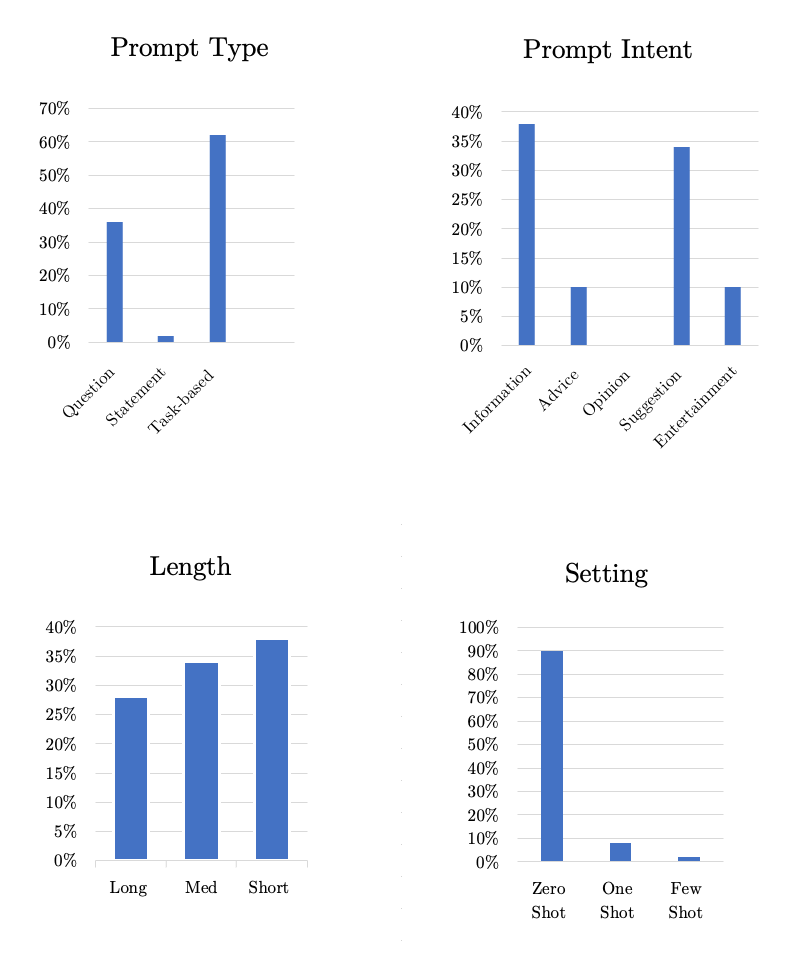
\includegraphics[width=0.4\textwidth]{images/barcharts1}
    \caption{ShareGPT Prompt Analysis Categories 1--4}
    \label{fig:chatgpt-categories-1}
\end{figure}
\begin{figure}[h]
    \centering
    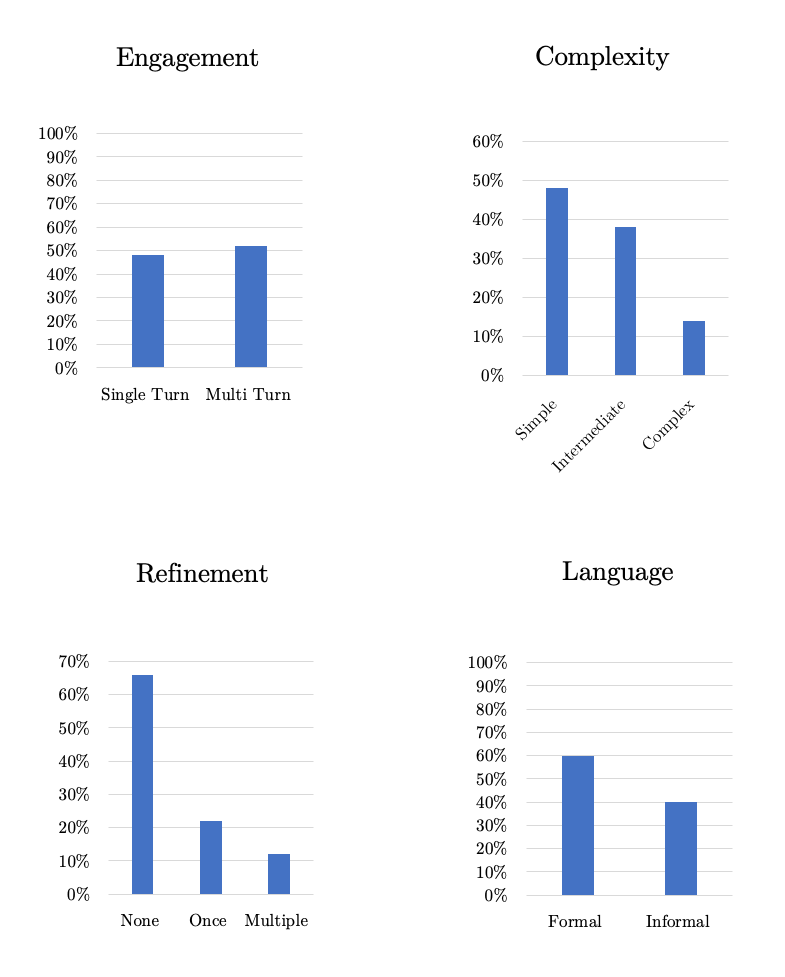
\includegraphics[width=0.4\textwidth]{images/barcharts2}
    \caption{ShareGPT Prompt Analysis Categories 5--8}
    \label{fig:chatgpt-categories-2}
\end{figure}
\begin{figure}[t]
    \centering
    \vspace{10.5mm}
    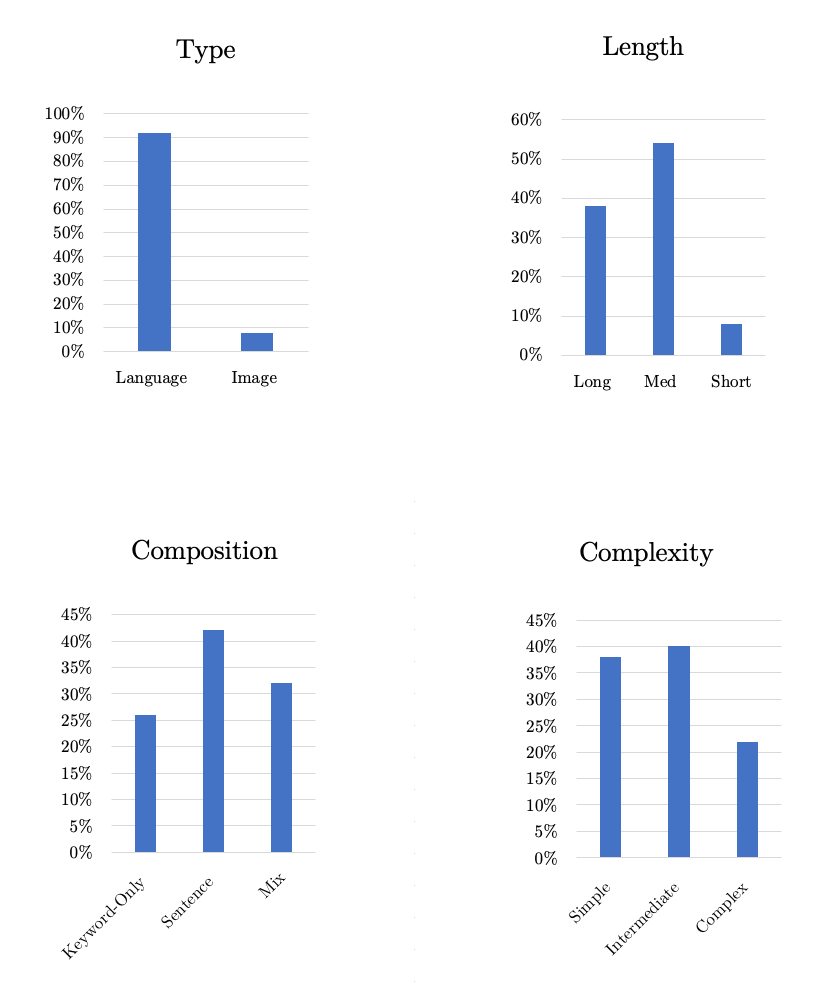
\includegraphics[width=0.4\textwidth]{images/barcharts3}
    \caption{Midjourney Prompt Analysis Categories 1--4}
    \label{fig:midjourney-categories-1}
\end{figure}
\begin{figure}[t]
    \centering
    \vspace{8.275mm}
    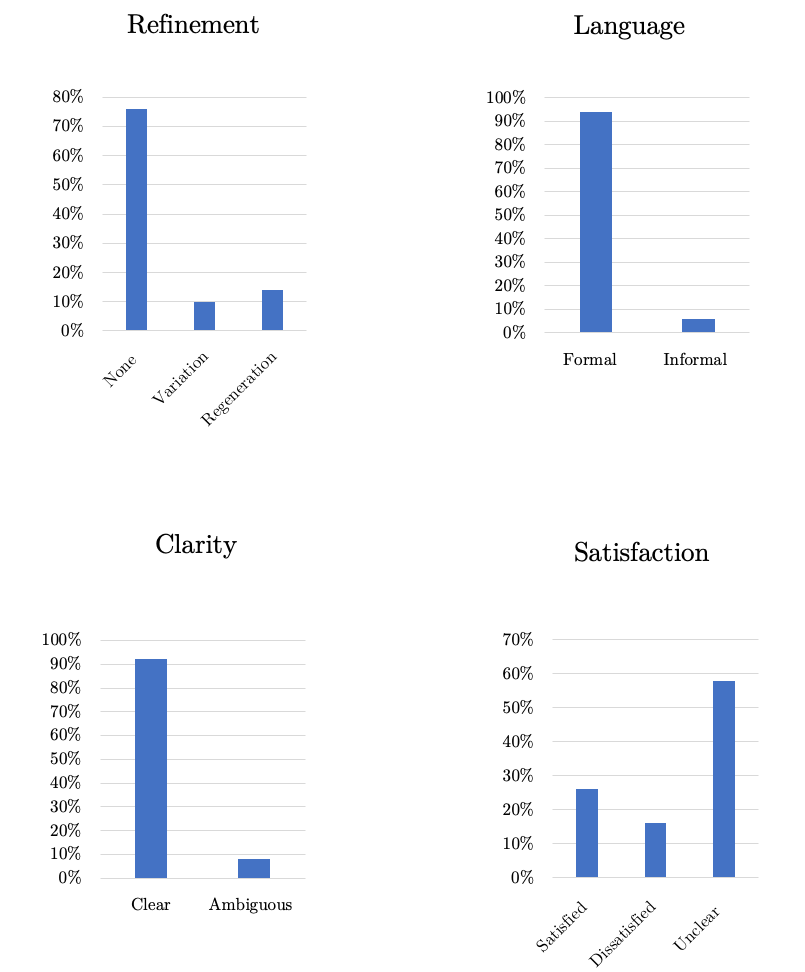
\includegraphics[width=0.4\textwidth]{images/barcharts4}
    \caption{Midjourney Prompt Analysis Categories 5--8}
    \label{fig:midjourney-categories-2}
\end{figure}

%\begin{figure}[T]
%    \begin{subfigure}[t]{0.3\textwidth}
%        \centering
%        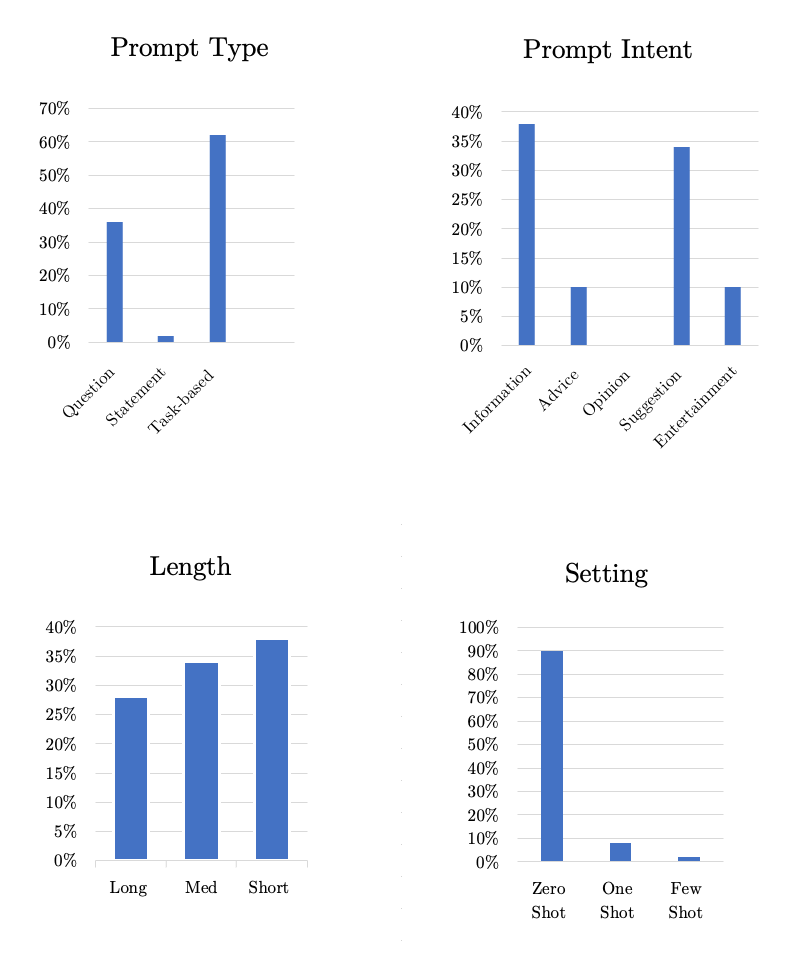
\includegraphics[width=0.2\textwidth]{images/barcharts1}
%        \caption{ShareGPT Prompt Analysis Categories 1--4}
%        \label{fig:chatgpt-categories-1}
%    \end{subfigure}
%    \hfill
%    \begin{subfigure}[t]{0.3\textwidth}
%        \centering
%        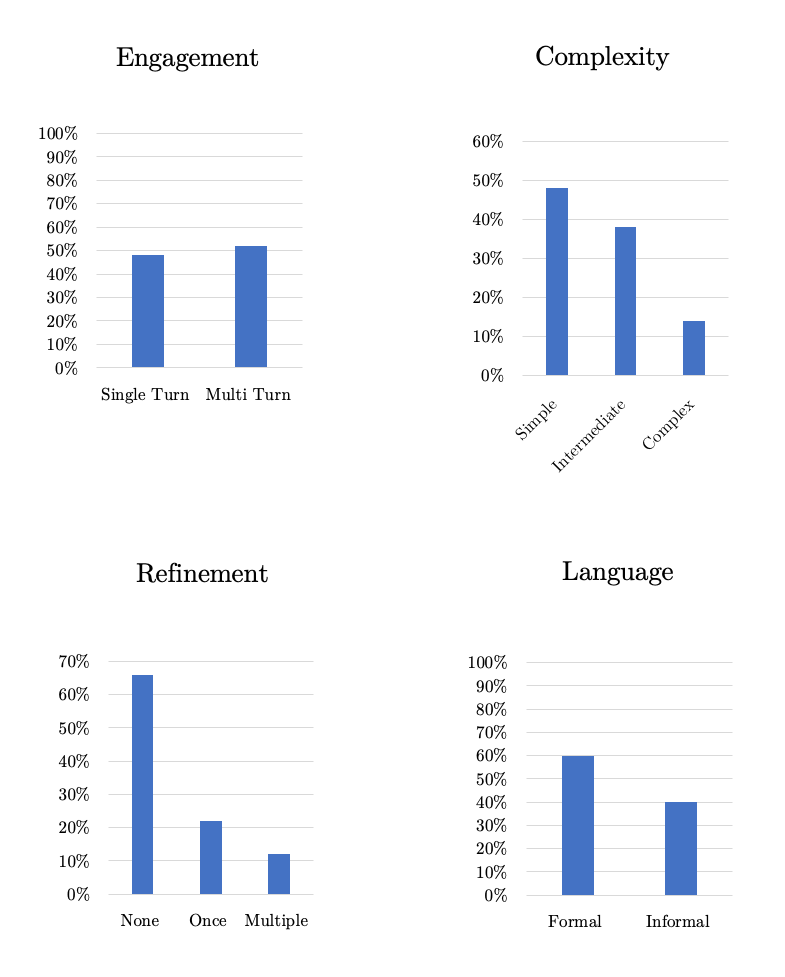
\includegraphics[width=0.2\textwidth]{images/barcharts2}
%        \caption{ShareGPT Prompt Analysis Categories 5--8}
%        \label{fig:chatgpt-categories-2}
%    \end{subfigure}
%    \vspace{0.5cm}
%    \begin{subfigure}[T]{0.475\textwidth}
%        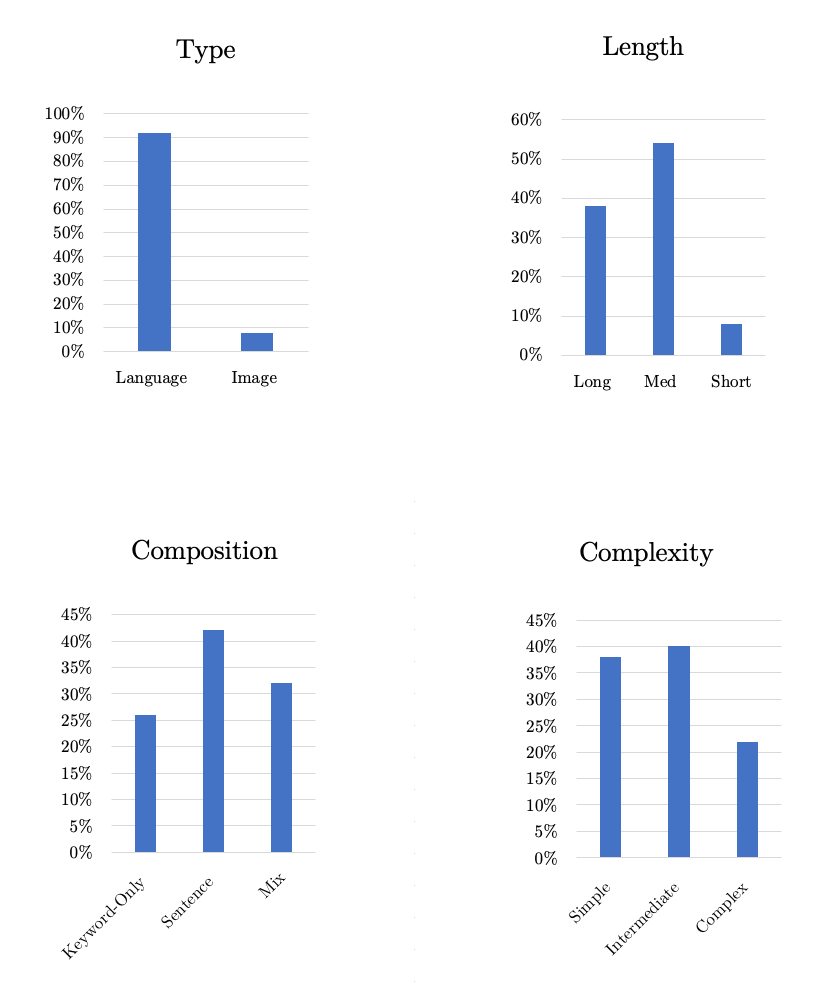
\includegraphics[width=0.2\textwidth]{images/barcharts3}
%        \caption{Midjourney Prompt Analysis Categories 1--4}
%        \label{fig:midjourney-categories-1}
%    \end{subfigure}
%    \hfill
%    \begin{subfigure}[b]{0.475\textwidth}
%        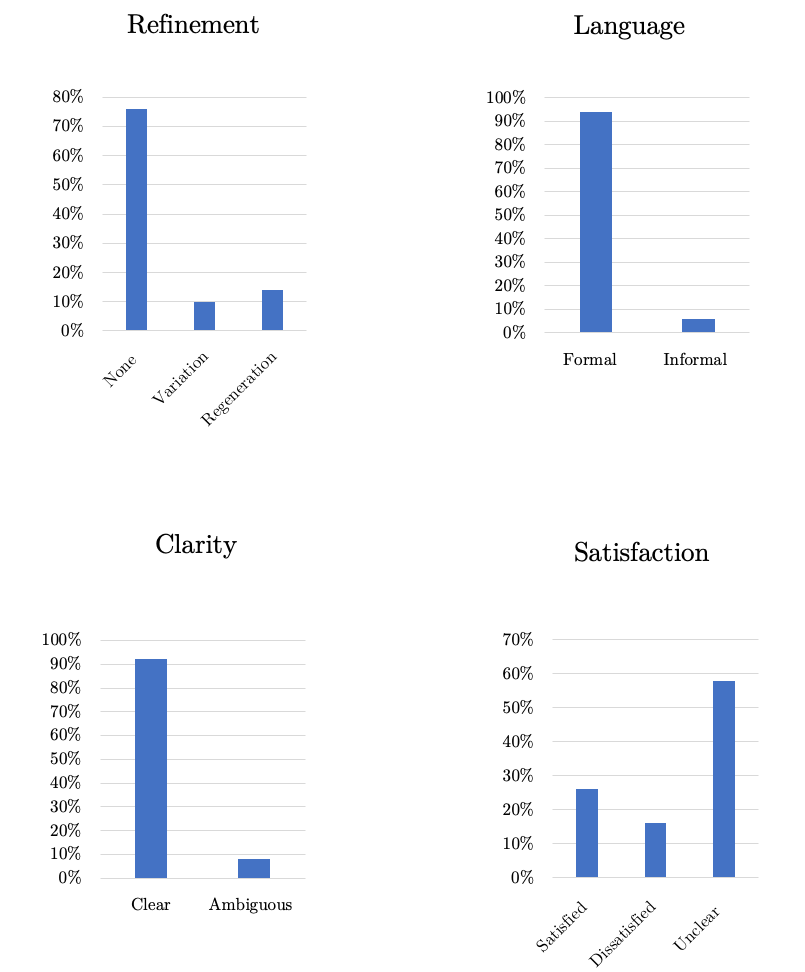
\includegraphics[width=0.2\textwidth]{images/barcharts4}
%        \caption{Midjourney Prompt Analysis Categories 5--8}
%        \label{fig:midjourney-categories-2}
%    \end{subfigure}
%\end{figure}



%%%%%%%%%%%%%%%%%%%%%%%%%%%%%%%%%%%%%%% BIBLIOGRAPHY
\clearpage
\bibliographystyle{ACM-Reference-Format}
\bibliography{bibliography}

\end{document}
\endinput
